\section{Aufgabe 6 - Stoppuhr}
\subsection{Entwurf}
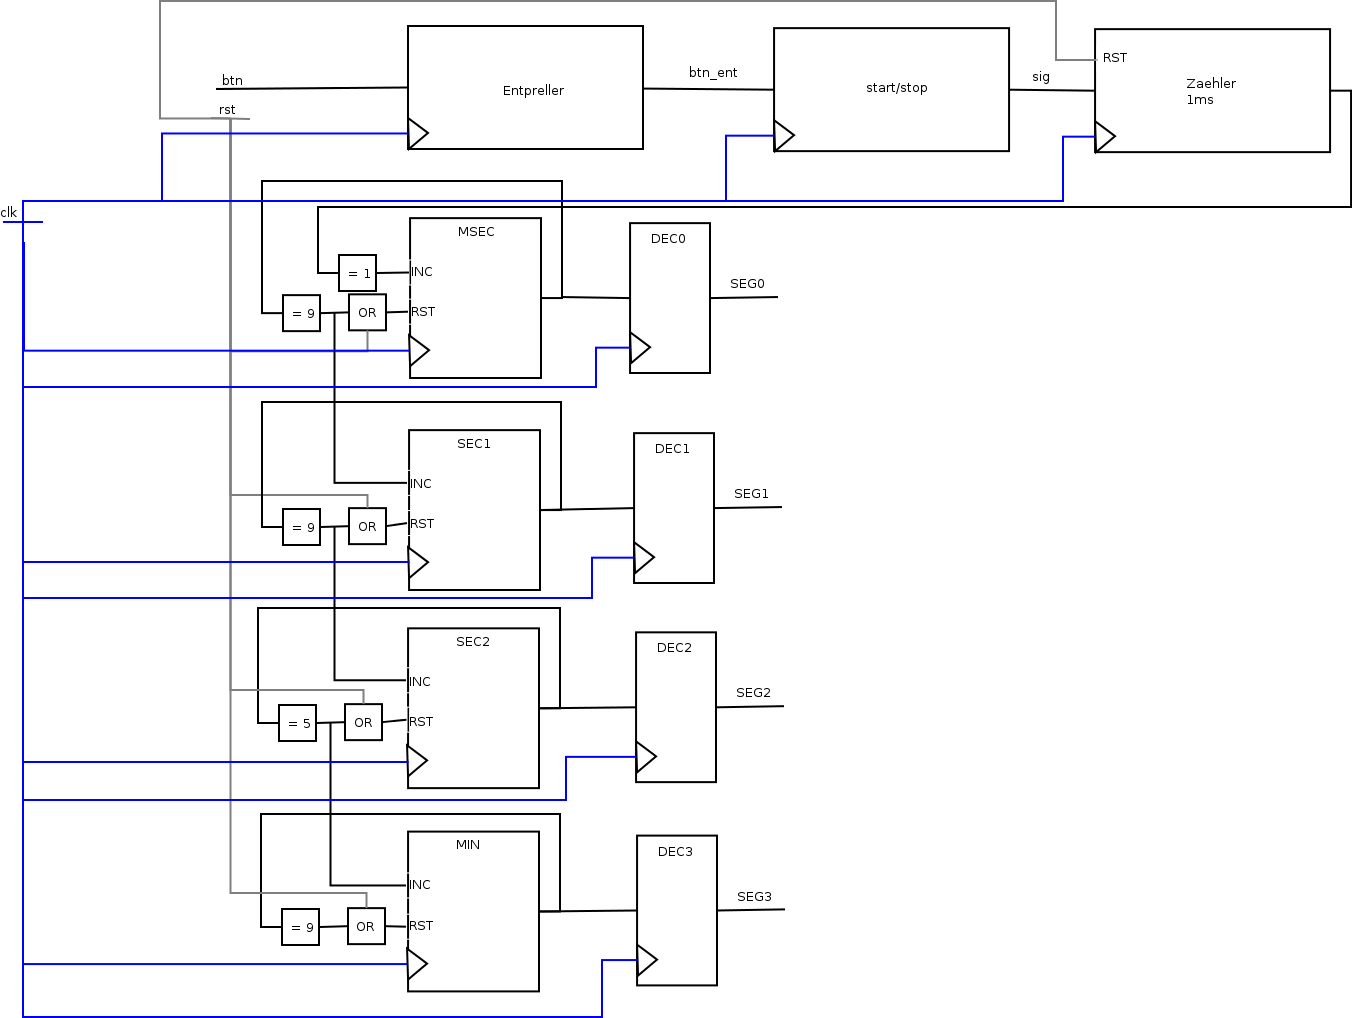
\includegraphics[width=1\textwidth]{resources/06-stopuhr.png}
	\newpage
	\paragraph{State-Machine-Charts}\hfill \\

		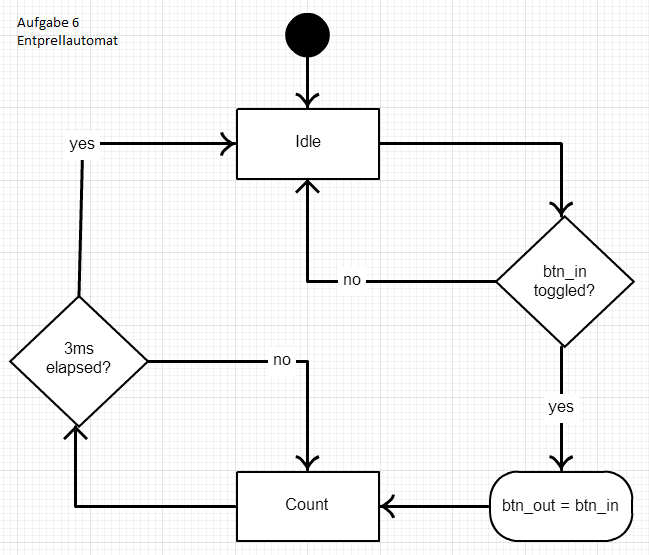
\includegraphics[width=0.8\textwidth]{resources/06-Entprellautomat.png}
		

		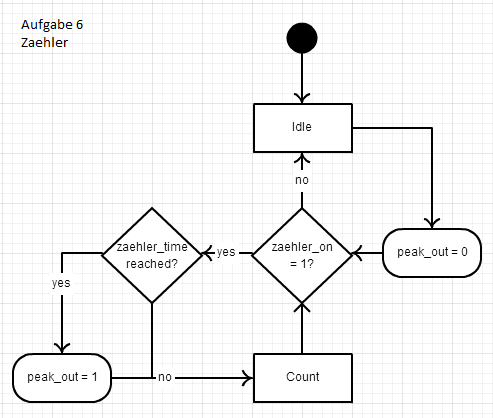
\includegraphics[width=0.7\textwidth]{resources/06-Zaehler.png}

		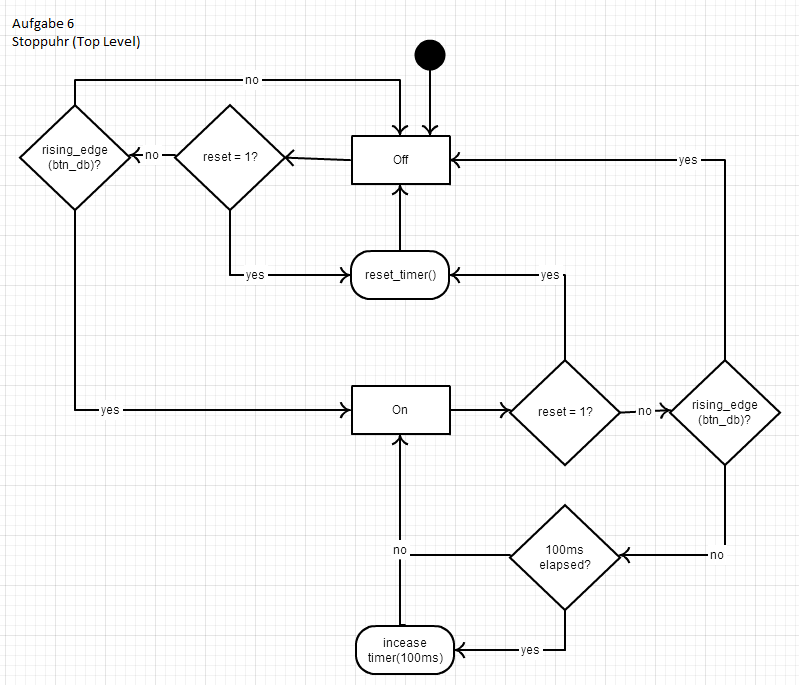
\includegraphics[width=0.7\textwidth]{resources/06-Stoppuhr.png}
 
	\paragraph{Kopplung} \hfill\\
	Es wird eine synchrone Automatenkopplung über die Ausgangssignale mit einem Taktsignal verwendet.
\subsection{Auswertung}
	\paragraph{Ressourcenbedarf}
	\begin{itemize} 
	\item 163 Logik-Elemente
	\item davon 121 dedizierte Logik-Elemente
	\item 35 Pins 
	\item maximale Taktfrequenz von 225 MHz
	\end{itemize}
